\documentclass[helvetica,narrow,openbib]{europecv}
\usepackage[T1]{fontenc}
\usepackage[a4paper,top=2cm,left=1cm,right=1cm,bottom=2cm]{geometry}
\usepackage{ifpdf}
\usepackage{bibentry}
\usepackage[italian]{babel}
\usepackage{url}
\ifpdf
    \usepackage[pdftex]{graphicx}
\else
    \usepackage{graphicx}
\fi
\usepackage{xcolor}

\renewcommand{\ttdefault}{phv} % Uses Helvetica instead of fixed width font
\renewcommand{\emph}[1]{\textbf{#1}}
\ecvlastname{Ziosi}
\ecvfirstname{Brunetto Marco}
\ecvaddress{via Ivancich n.17, 30174, Chirignago (VE)}
\ecvtelephone{(+39) 3474958152}
\ecvemail{brunetto.ziosi@gmail.com}

\ecvnationality{Italian}
\ecvdateofbirth{03/05/1985} % FIXME Solo per application in Europa

\thispagestyle{empty}

\begin{document}
\selectlanguage{italian}
%\ecvfootnote{Curriculum Vitae of Brunetto Marco Ziosi}

\begin{europecv}
%\ecvpersonalinfo[20pt]
\ecvsection{\textcolor[rgb]{0.35,0.35,0.35}{Personal information}}
\ecvitem{Name}{{\bf Brunetto Ziosi}}
\ecvitem{Email}{brunetto.ziosi@gmail.com}
\ecvitem{Phone}{(+39) 3474958152}
\ecvitem{Address}{Via Castellana 221, 20174, Zelarino (VE)}

\ecvitem{Website}{\texttt{brunettoziosi.eu}}
\ecvitem{LinkedIn}{\texttt{https://www.linkedin.com/in/brunettoziosi}}
\ecvitem{Public repositoris}{\texttt{github.com/brunetto}, \texttt{gitlab.com/brunetto}}

\ecvsection{\textcolor[rgb]{0.35,0.35,0.35}{Experience}}
\ecvitem{\textcolor[rgb]{0.35,0.35,0.35}{\bf 2015/09 - present}}{\bf Full stack developer at Pixartprinting - a Cimpress company}
\ecvitem{\textcolor[rgb]{0.35,0.35,0.35}{2015/01-2015/07}}{Fellowship at National Institute for Astrophysics (INAF - OAPd)}
\ecvitem{\textcolor[rgb]{0.35,0.35,0.35}{2012-2013}}{Teaching assistant: Mathematical Analysys, Python Lab - Department of Physics and Astronomy, University of Padova}

\ecvsection{\textcolor[rgb]{0.35,0.35,0.35}{Education}}
\ecvitem{\textcolor[rgb]{0.35,0.35,0.35}{2012-2015}}{{\bf PhD in Astrophysics} - Department of Physics and Astronomy, University of Padova}
\ecvitem{\textcolor[rgb]{0.35,0.35,0.35}{2007-2011}}{Master Degree in Astronomy - Department of Physics and Astronomy, University of Padova}
\ecvitem{\textcolor[rgb]{0.35,0.35,0.35}{2004-2007}}{Bachelor Degree in Astronomy  - Department of Physics and Astronomy, University of Padova}

\ecvsection{\textcolor[rgb]{0.35,0.35,0.35}{Courses and Workshops}}

\ecvitem{\textcolor[rgb]{0.35,0.35,0.35}{2016}}{
- Microservices with Docker and AWS

- Continuous integration, Jenkins

- Test Driven Development
}

\ecvitem{\textcolor[rgb]{0.35,0.35,0.35}{2014}}{
- Amazon Web Services Cloud School

- Tools and Techniques for massive data analysis

- Perspectives of GPU computing in Physics and Astrophysics
}

\ecvitem{\textcolor[rgb]{0.35,0.35,0.35}{2013}}{
 -  Workshop on High Performance Scientific Computing
 
 - PhD Summer School on High Performance Scientific Computing
}
\ecvitem{\textcolor[rgb]{0.35,0.35,0.35}{2012}}{
 - Summer School of Parallel Computing
 }
 \ecvitem{\textcolor[rgb]{0.35,0.35,0.35}{2011}}{
 - PhD Summer School on Algorithms and Architectures for Computational Science and Engineering

 - Workshop on Visualization of Large scientific Data
 
 - Python for computational science

 - Introduction to GPGPU and CUDA programming
}

\ecvsection{\textcolor[rgb]{0.35,0.35,0.35}{Skills}}
\ecvitem{OSs}{Linux, MacOS, Windows}
\ecvitem{Scripting/Programming/Web}{Go, Python, PHP, JS, HTML5, CSS}
\ecvitem{Data Analysis/Plotting}{Veusz, Matplotlib/Pylab}
\ecvitem{Graphics}{Inkscape, Gimp, ImageMagick}
\ecvitem{Presentation}{Beamer, Sozi/Inkscape, Prezi, PowerPoint, Javascript based (Remark)}
\ecvitem{Misc}{Docker, Git, SVN, Bazaar, MySQL, MongoDB, LaTeX, Markdown}

\ecvsection{\textcolor[rgb]{0.35,0.35,0.35}{Interests}}
\ecvitem{}{

Telegram Bot APIs

Volunteering with A.G.E.S.C.I. (Wood Badge 17/03/2012-356) and Protezione Civile (Civil Defense)

Digital Photograpy | Piano and guitar | Travelling

Mapping and geo-data manipulation (OpenStreetMap project)
}

%\ecvsection{\textcolor[rgb]{0.35,0.35,0.35}{Signature}}
%\ecvitem{}{
%\begin{flushright}
%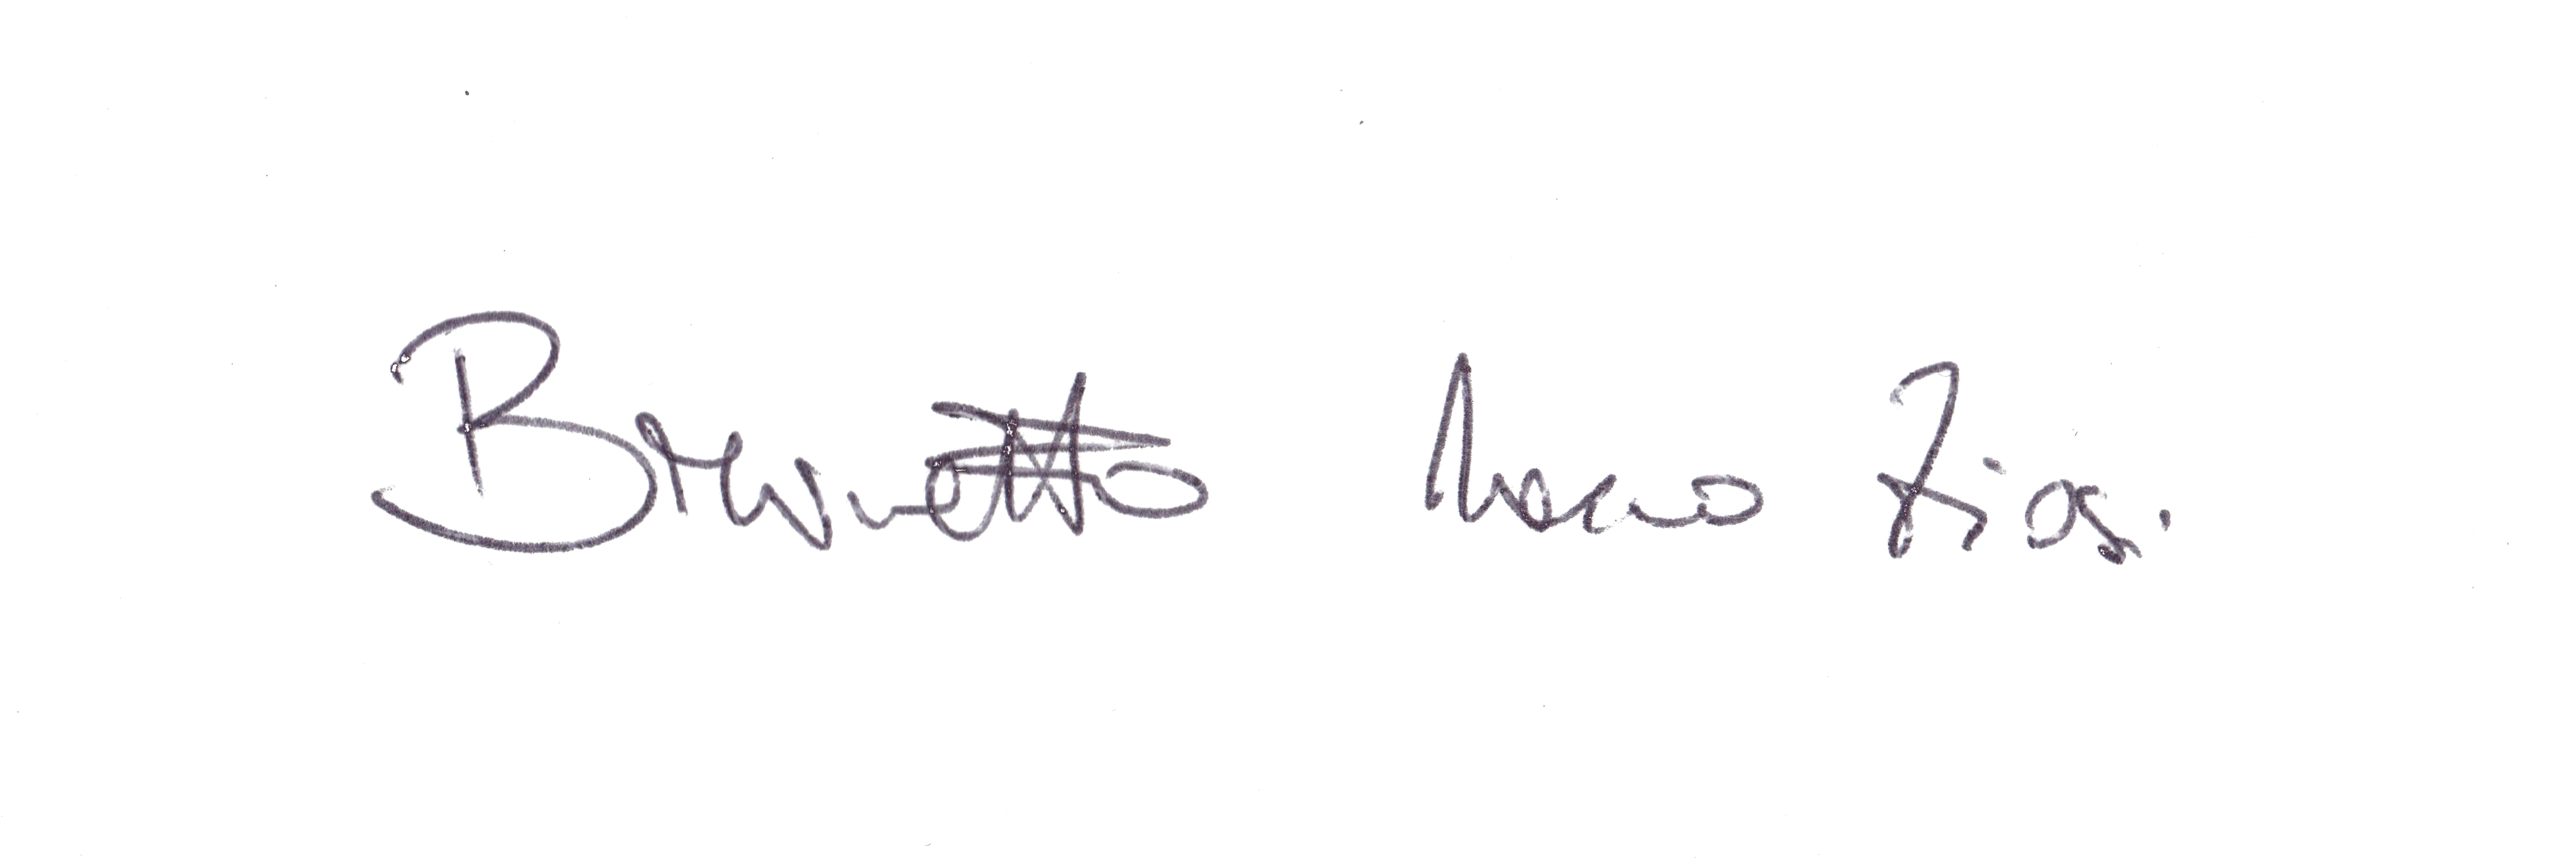
\includegraphics[width=9cm]{firma}
%\end{flushright}
%}

\end{europecv}
\end{document} 
